\documentclass[11pt]{article}
\usepackage{fancyhdr, graphicx, xcolor, caption, subcaption}
\usepackage{wrapfig}
\usepackage[section]{placeins}
\renewcommand{\headrulewidth}{0pt}

\pagestyle{plain}
\title{{Intermediate Report}}
\date{}
\author{team\_we\_got\_this}
\begin{document}
	\maketitle
	\thispagestyle{fancy}
	\section{Introduction}
	In this report we will discuss the initial progress of our group project. 
	In first section we will discuss the design and policies of the simulation and in the latter section we will discuss how the group is organised.
	
	
	\section{Project Description}
	
	\subsection{Overview of our Simulation}
	\begin{figure}
		\begin{subfigure}{.45\textwidth}
		\centering
		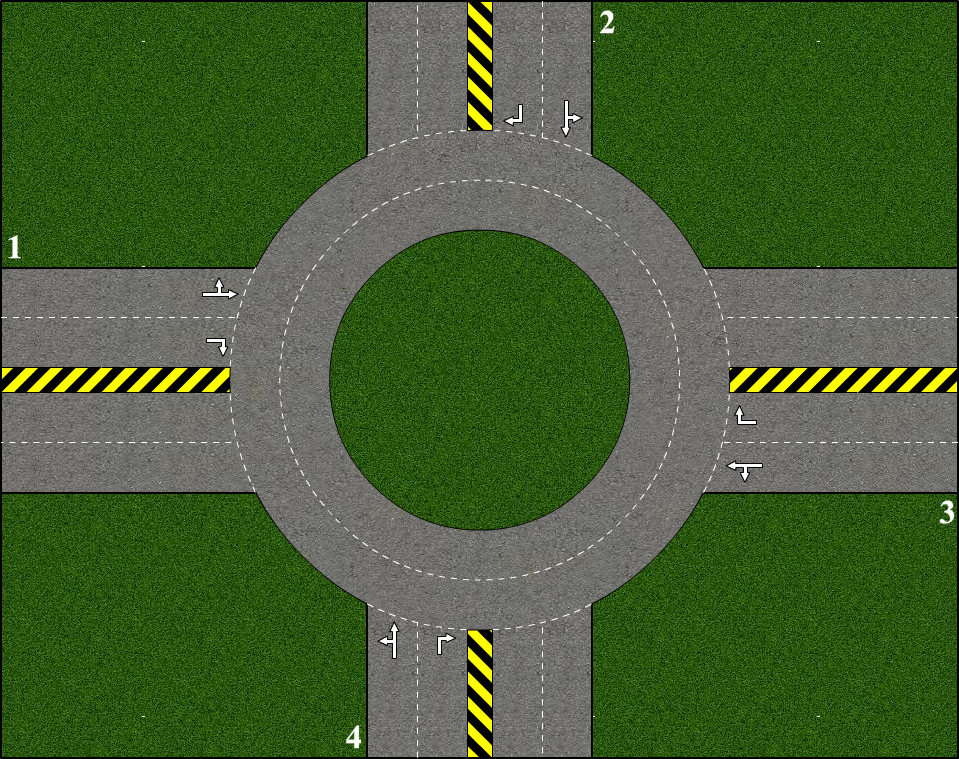
\includegraphics[width=0.65\textwidth]{Roundabout2}
		\caption{Our roundabout design}
		\label{RoundaboutDesign}
		\end{subfigure}
		\begin{subfigure}{.45\textwidth}
		\centering
		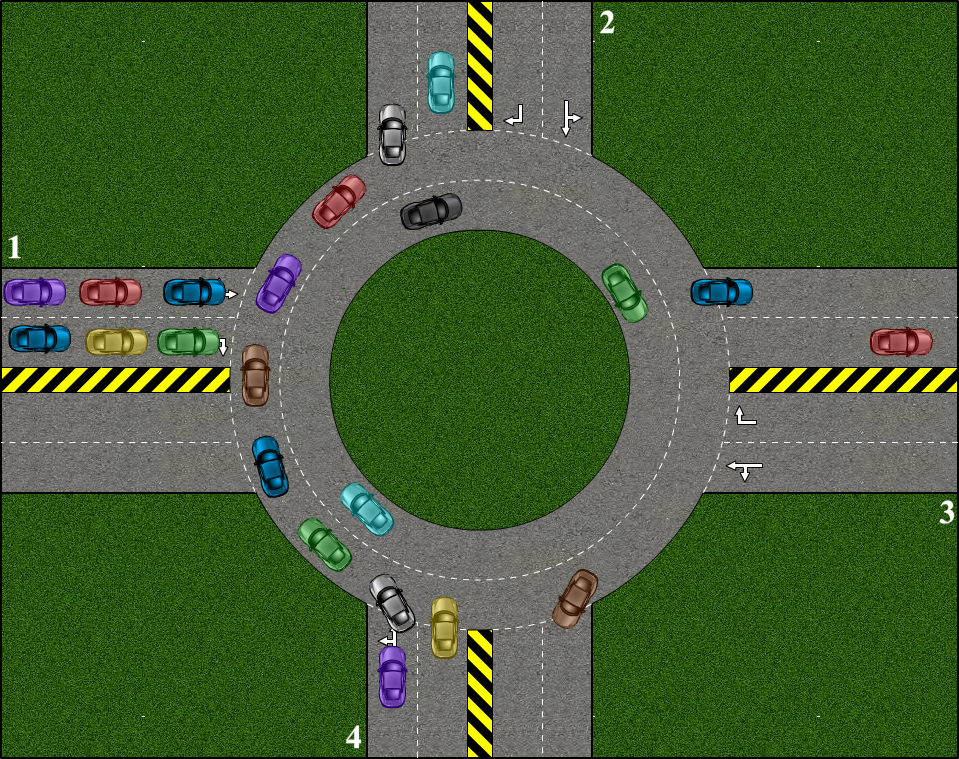
\includegraphics[width=0.65\textwidth]{SteadyFlow}
		\caption{Image of our blocked roundabout}
		\label{Steadyflow}
		\end{subfigure}
	\end{figure}
	Our group proposes to build a four junction roundabout with multiple lanes (see figure \ref{RoundaboutDesign}) and to introduce policies and road layouts loosely based around existing roundabouts in London.
	 Originally our design included traffic lights but within two weeks we had working traffic lights on our test simulation.
	  Hence, it was decided that it would more challenging to build a roundabout without traffic lights, as our cars would then need to be intelligent enough to know when to give way to other cars already on the roundabout. 
	  We aim to also allow users to change the probability of cars coming from each junction, entering the roundabout, to allow users to accurately measure real life scenarios.
	   For example, if there was a heavy flow of cars from one junction, this will stop cars from the junction to the left of it entering the roundabout as they will have to give way (see figure \ref{Steadyflow})
	
	\pagebreak
	If we could succeed in implementing the give way policy we would then create our own scenario, introduce
	traffic lights to analyse network flow and policies to improve this flow. 
	We will then analyse how many cars enter the roundabout from each junction per minute. 
	Our system would give users control of the time duration of the lights so that we could allow lights to be green for a longer duration at junction where the traffic flow is heavy. 
	As an optional attribute to our system we would like to implement traffic lights which are dynamic and will change colour based on the number of cars passing through instead of time elapsed. \\
	
	
	\begin{tabular}{ | l | c | r | }
		\hline
		\multicolumn{3}{|c|}{Project Timetable}  \\ \hline
		Date & Description of Implementation & Status \\ \hline
		22/01/15 & Basic model with moving cars &  Achieved \\ \hline
		29/01/15 & Collision detection and avoidance & Achieved \\ \hline
		16/02/15 & Working Basic Cellular Automation model & Pending \\ \hline
		04/03/15 & Roundabout & Pending \\ \hline
		21/03/15 & Multi-lane roundabout & Pending \\ \hline
		
	\end{tabular}\\\\
	
		\noindent As a group there were several different approaches that we thought were viable. 
		We decided to explore each option and an overview of each is discussed in sections 2.2 and 2.3
		\
	\subsection{Design Approach 1: Using a Matrix}

	
	The first option we trialled was building our system in ActionScript 3.0 built on a hexagon matrix. 
	In this model we used coordinates to track the position of cars on the matrix as this would allow us to prevent collisions. 
	We used a hexagon matrix as we thought it would better suit the shape of the roundabout, however in the trial of the model we decided a hexagon grid was an unnecessary complication. 
	
%	In this model we have traffic lights which have a green signal for different directions and have cars which can respond to this, i.e. if a light was green for straight ahead only and the car at the light wanted to turn left, the car would not go. The cars could not respond to other cars on the road and hence if a car was travelling at a faster speed than the car in front of it, it would go through it.
	
	The second option is based on a cell automation model \cite{namekawa2005general}. 
	In this model each cell of a matrix is given attributes and properties. 
	The attributes will include the width, height and type of cell whilst the properties will give information on whether the cell is occupied by a vehicle. 
	The most important feature we will include in each cell is information on its neighbouring cell so that cars can make dynamic decisions about where they will go in the next tick on the simulation.
	
	
	\subsection{Design Approach 2: Using Equations}
	\FloatBarrier
	
	
    The third model was the first working simulation the group created (see figure \ref{NurScreenshot}). 
    It is built by recolouring pixels every 30 milliseconds to show movement of the cars across the map. 
    We had this working model running quickly, but we questioned whether it would be dynamic enough to adapt to our growing plans. 
    In particular, we were concerned that this naive approach would hold us back as we tried to develop a multi-lane roundabout where cars would need to change lanes. 
    Originally this model had issue with collisions but it now has a level of intelligence - cars can respond to other cars in front of them by changing lanes. 
    They also know not to overtake on the left. 	
\begin{figure}
	
	\centering
	\begin{subfigure}{.35\textwidth}
		\centering
		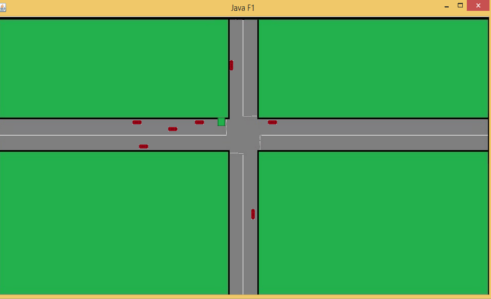
\includegraphics[width=0.9\textwidth]{ScreenShotNurSim}
		\caption{Screenshot of  our model }
		\label{NurScreenshot}
	\end{subfigure}
	\begin{subfigure}{.35\textwidth}
		\centering
		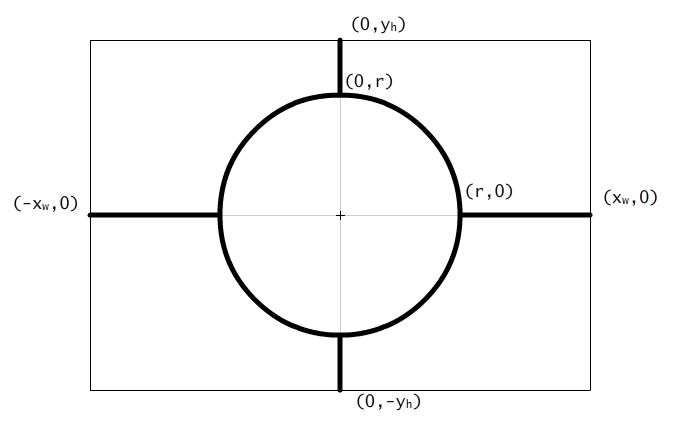
\includegraphics[width=0.9\textwidth]{KimsModel}
		\caption{Sample graph for Our Continuous Model}
		\label{KimModel}
	\end{subfigure}
\end{figure}	
%	\FloatBarrier
%	\begin{figure}[h]
%		\centering
%		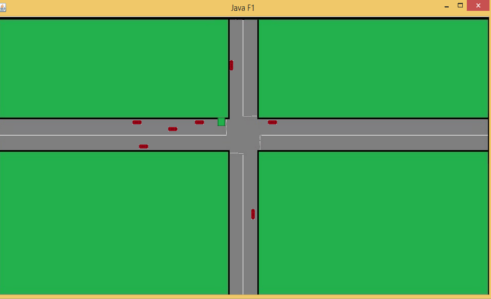
\includegraphics[width=0.45\textwidth]{ScreenShotNurSim}
%		\caption{Screenshot of our first working model}
%		
%	\end{figure}

%	In this system the map is on a coordinate system and a car travelling at say $30 m/s$ from west to east would increase its x-coordinate by 30 in the next time frame and similarly for other movements. 
%	The model worked by changing the colour of pixels as a car moved  current simple crossroad but as our system developed in to a multi-lane roundabout this naive approach would begin to hold us back.	
%	Originally this model had an issue with collisions as our cars did not know of the existence of others. This problem was fixed by each car first checking if its new coordinates will intersect with the coordinates of another car already on the map. If it does intersect then car will try to change into the right lane. If the right lane is occupied or if it is already in the right lane the car will stay where it is, following the car in front. Our cars also only overtake from the outside and know not to overtake by crossing into the lane for traffic flowing in the opposite direction. We would like to the adapt the system so that a car and can alert the car in front that it is moving too slow and have the other car receive this message and react according just like in real life. This has the possibility to be extended into speed restriction for each lane, i.e. the maximum speed in the left lane being $30m/s$ whilst the right lane could be the fast lane with a maximum speed of $60m/s$
	The final approach we considered was a continuous model in which our map was represented by several parametric equations (see figure \ref{KimModel}). 
	Although this approach would allow us to accurately calculate where each car is at any time, we decided this implementation would be unnecessarily time-consuming.  
	
%	\begin{figure}
%		\centering
%		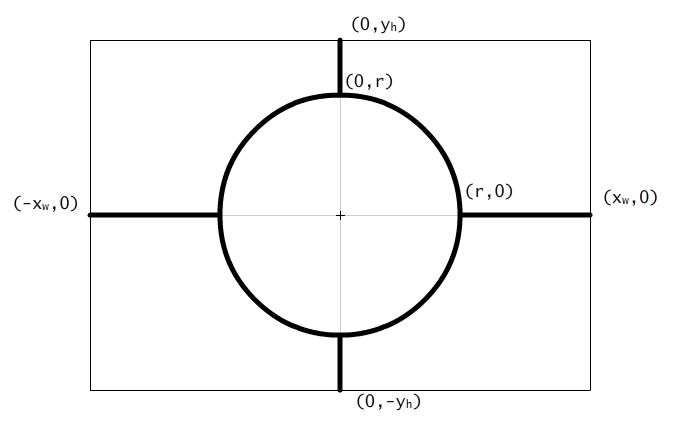
\includegraphics[width=0.45\textwidth]{KimsModel}
%		\caption{Sample graph for Our Continuous Model}
%	\end{figure}

\subsection{Final Implementation Choice}

	
	
	
	\section{Project Organisation}
		At the start of our project our group decided to meet for two hour meetings twice a week. 
		The weekly meeting slots are at a set time but this caused some issues, hence we are now aiming to be more flexible with the meeting times. 
		Now that we have decided on the final approach of our system, we are having separate meetings to discuss individual areas of the project, i.e meetings for the software engineers. 
		Whilst we all have an active say in all areas of the project, we all have different focuses. 
		Rochelle is project coordinator and administrator; Zaki, Anton, and Nur are software developers; and Kim is graphics coordinator and assistant software developer. 
		In the peer assessment we plan to give everyone equal marks as we all have pre-defined and necessary roles in the project. 
		We are trying to compromise on smaller issues while voting on any large issues. 
		 
		One of our difficulties thus far has been using GitHub. 
		It has been very challenging for all of us to learn how to use this new platform. 
		Much of our project so far has been diagrams or pictorial representations of what we plan to do. 
		As we are unsure what file types git allows, we have been using a shared Dropbox folder for our group. 
		We have now set a deadline(16/02) for each member of the group to learn how to use git. 
		It was agreed that each week by Sunday at 6pm, we will all push what we have been working on that week to the repository, creating new branches where necessary. 
		
		The biggest challenge we have faced as a group is communication. 
		We could not agree as a group what we to use to communicate with each other and as a result there were messages which were not received by every member of the group. 
		We have now agreed to all use the application 'Slack' as our primary means of communicating. 
		
		We are following a waterfall structure for our group as it is simple and clear approach which all members can follow. 
		We are using UML diagrams to set out clear specifications for our software developers. 
		This will allows us to work on separate areas of the program and then merge the components.  
	
%	Our group agreed to meet for weekly two hour meetings at the start of our project. The weekly meeting slots are at a set time but this caused some issues, hence we are now aiming to be more flexible with the meeting time. Also now we have decided on the final approach of our system, we have agreed to have separate meetings to discuss individual areas of the project, i.e meetings for the software engineers. Whilst we all have a active say in all areas of the project, we all have different focuses. Rochelle is project coordinator and administrator; Kim is Graphics coordinator/ assistant software engineer; and Zaki, Anton and Nur are software developers. In the peer assessment we plan to give everyone equal points as we all have pre-defined and necessary roles in the project. We try to compromise on smaller issue and then just vote on any large issue.  
%	
%	In the peer assessment we plan to give everyone equal points as we all have pre-defined and necessary roles in the project.
		

\bibliographystyle{plain}
\bibliography{references.bib}
	
\end{document}